\section{Evaluation}
\label{evaluation}
We perform experiments to answer two main questions: (a) How much performance improvement is possible through carefully tuning the batch-size $B$ and
the sub-batch-size $b$?  (b) Can we develop a performance model from the experimental data, to generalize our results for automatic
optimization by a compiler
optimizer, for an arbitrary packet processing pipeline. We develop a preliminary model to explain our current results. We have
integrated our model into P4C
to automatically optimize the applications used in this paper.

\subsection{Evaluation Setup}
\textbf{Hardware}: Dell Poweredge R430 Rack Server, based on Haswell architecture. This server has two sockets occupied with Intel Xeon E5-2640 
v3\cite{xeon} processor. Each processor has 8 physical and each core is capable of running at 2.60 GHz. Cores on a socket share 20 MB cache. Sockets are connected with 2 QPIs(Quick Path Interconnect), each capable of 8 GT/s. Two dual port NICs,1 Intel x520 and 1 Intel x540, are connected to Socket 0 through PCIe 2.0 and each port can work at 10Gbps. Total main memory available is 64 GB, spread across two sockets in a NUMA fashion.
\\
\textbf{Software}: Ubuntu 14.04 LTS operating system with 4.4.0-59 Linux kernel version. We are using DPDK version 16.07 with IXGBE poll mode driver to
interact with the underlying NICs. 
\\
\textbf{Traffic Generator}: We are using same hardware and software on both the servers and Pktgen-DPDK\cite{pktgen} version 3.1.0 to generate different kind of packets for different applications used in the experiments. Pktgen-DPDK\cite{pktgen} can generate the 64 bytes packet size traffic at line rate i.e 14.8 Mpps for 10 Gbps port. We are able to generate traffic at 59 Mpps for four ports with 64 bytes packet size. We have extended Pktgen-DPDK\cite{pktgen} to put random source and destination address depending on the application.
\\
\textbf{Methodology}: We use packet-processing pipelines developed in P4\cite{Bosshart:2014:PPP:2656877.2656890} as our test applications. We have extended the P4C\cite{Laki:2016:HSP:2934872.2959080} compiler to generate code with batching, sub-batching and prefetching. P4C\cite{Laki:2016:HSP:2934872.2959080} generates C-code that can be run with the DPDK\cite{DPDK} framework, which is then compiled into an executable using GCC. Unless otherwise specified, all
applications are tested with minimum-sized packets (64 bytes), to test the limits of the system.
\\
\textbf{Applications}: Our applications are similar to the ones used in \cite{189006}, to allow head-to-head comparison of performance results:
\begin{enumerate}
\item \textbf{Layer 2 Switch}: Two hash tables are used to store the mapping between SMAC/DMAC and the forwarding port. Each packet goes through two lookup stages, one for SMAC and another for DMAC. By default, we assume 16 million entries in both tables (as also used in \cite{189006}), unless otherwise specified.
%We are using Intel DPDK's implementation for various hash table operations.
\item \textbf{IPV4 Forwarding}: A longest-prefix match (LPM) lookup is performed on the destination IP address to get the forwarding port.
%We are using Intel DPDK's implementation for LPM related operations for IPv4 Forwarding and IPv6 Forwarding application.
We populate the forwarding table with 527,961 prefixed, as also used by \cite{189006}.
\item \textbf{IPv6 Forwarding}: A longest-prefix match lookup is performed on the destination address to find the egress port. We populate the DPDK LPM table with 200,000 random entries with the length between 48 to 64, as also done in \cite{189006}. Through Pktgen, we generate packets with destination address randomly picked from these 200,000 entries. The minimum packet size for this application is 78 bytes and not 64 bytes.
\item \textbf{Named Data networking}: A hashtable lookup is used to map a string URL to a forwarding port.
%implemented by DPDK.
We use the URL dataset given in \cite{DBLP:conf/globecom/ZhangWYLL13}. Using Pktgen, we transmit packets containing URLs generated randomly from our dataset. We use 32 bytes URLs in our packet headers, as also done in \cite{189006}.
\item \textbf{L2 forwarding with encryption and decryption}: We use the L2Fwd-Crypto\cite{l2crypto} application available as a part of the DPDK source code. The application performs encryption and decryption based on the input parameters and it then forwards the packet on Layer 2 with static port mapping. Unlike other applications, which are largely memory-bound, this application is compute-bound.
\end{enumerate}

\subsection{Performance improvements achievable through batching and sub-batching}
\label{batchingandprefetching}
\begin{figure}[ht]
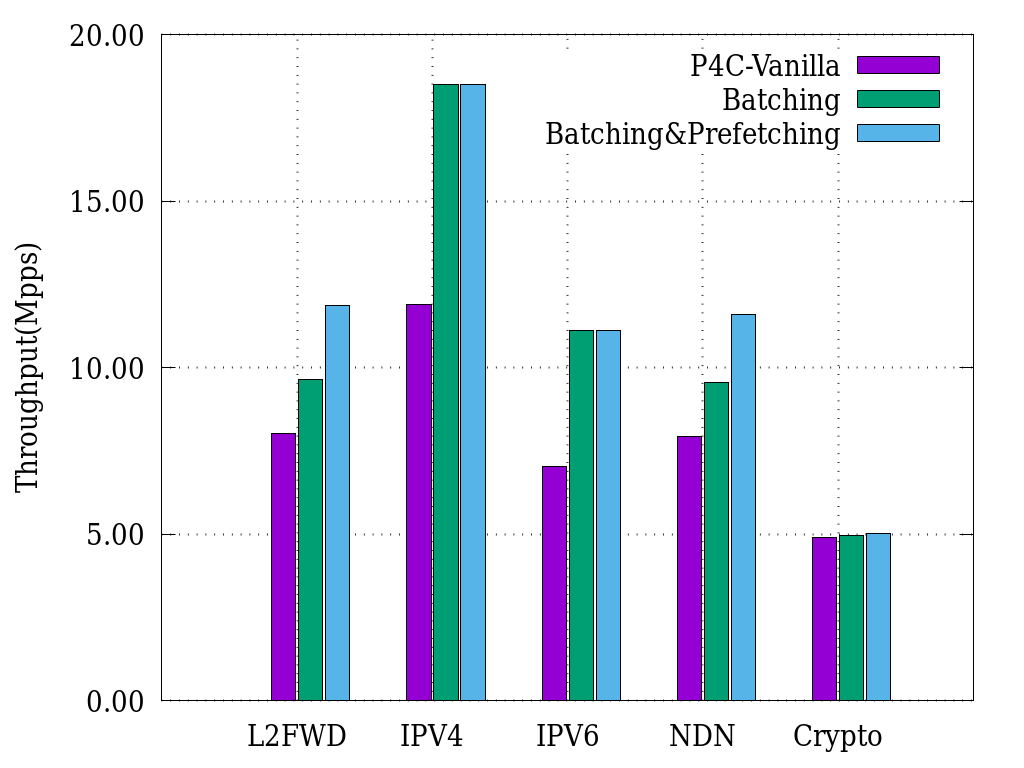
\includegraphics[width = \linewidth]{Figures/effectofbatching.png}
\caption{Effect of batching and prefetching}
\label{fig:batchingandprefetchingfigure}
\end{figure}
We added batching and sub-batching support to P4C, and show results for batch-size $B=32$
in Figure~\ref{fig:batchingandprefetchingfigure}. The ``{\tt Batching}'' results represent the case when sub-batching
is disabled (i.e., sub-batch-size $b=1$), while the ``{\tt Batching\&Prefetching}'' results represent the case
when sub-batching (and prefetching) is enabled and set to its maximum possible value, i.e., sub-batch-size $b=32$.
We later discuss the sensitivity of
throughput to changing $B$ and $b$.
For L2 forwarding, batching improves the performance by 20\% and sub-batching further improves the performance by an additional 23\%. Similarly
for NDN, batching alone improves the performance by 20\% and sub-batching results in an additional performance gain of 21\%.
Using $B=32$ and $b=32$ for IPv4 and IPv6, we obtain a performance gain of 55\% and 57\% respectively.
For a compute-intensive application like L2Fwd-Crypto, the performance improvements are much smaller.

\subsection{Sensitivity of Throughput to $B$}
We use the L2 forwarding application to demonstrate the effects of changing application behavior on the optimal
values for $B$ and $b$. We use the L2Fwd application with five different sizes of the lookup table. The size of
the lookup table approximately represents the working set of the application. If the table fits in the caches,
then the application is largely compute bound and has few accesses to the main memory. On the other hand, if the
table is much larger than the last-level cache, then almost every random table access will result in an access to
the main memory. Consequently, the changing application behavior results in a change in the value of the
optimal $B$ and $b$, required for optimal throughput.

Figure~\ref{fig:tablesize} plots the results for throughput for different table sizes and batch-sizes $B$. The solid
line represents the case when the sub-batch-size $b$ equals the batch-size $B$, i.e., $b=B$. The dotted line represents
the case when the sub-batch-size $b=1$, i.e., no sub-batching.

There are a few conclusions to draw from this plot: (1) Expectedly, throughput is generally higher
for smaller tables than for larger tables. (2) For all table sizes, the throughput usually increases with
increasing $B$ for $B<128$, due to better exploitation of DMA bandwidth. (3) A batch-size beyond 128, usually results in
decreased throughput due to greater stress on the caching subsystem. (4) Sub-batching improves the throughput
for larger table-sizes, but does not improve throughput for smaller table sizes. This is expected
because sub-batching benefits from memory-level parallelism. For small table-sizes, the main-memory
accesses are few, and so the benefit of sub-batching is little. We discuss this in more detail
in our next experiment. (5) $B=32$ provides near-optimal results across all configurations of the
L2 forwarding application.

\begin{figure}[ht]
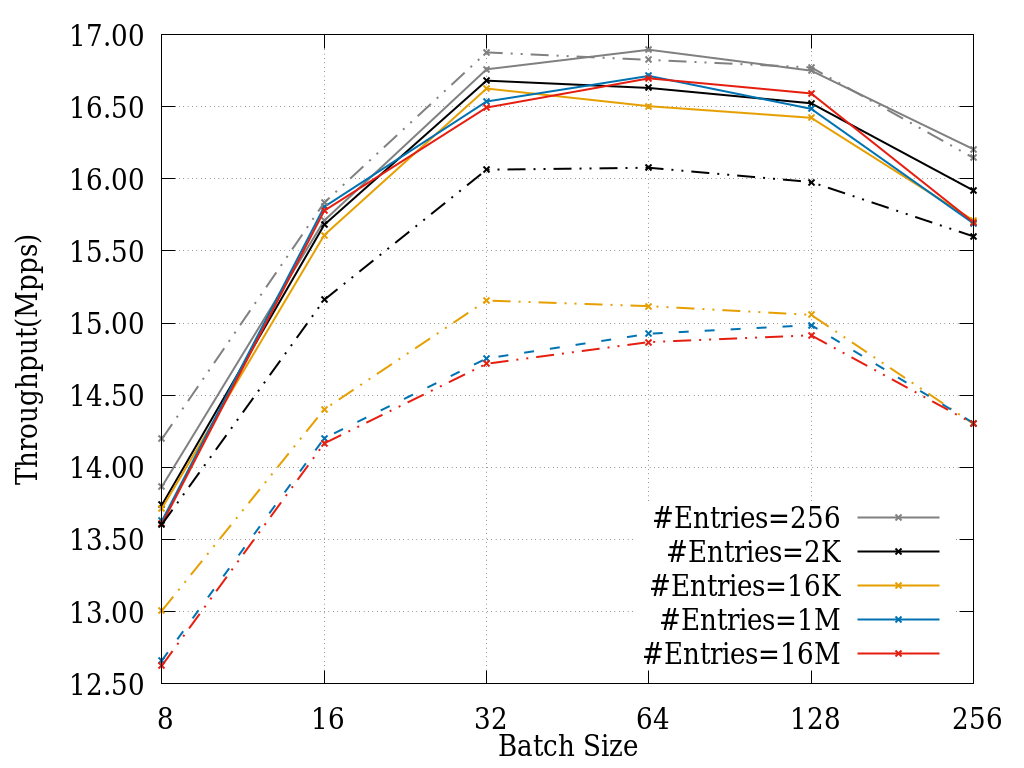
\includegraphics[width = \linewidth]{Figures/TableSizeVsbatchSize.png}
\caption{The effect of batch-size $B$ on application throughput, for five different configurations of the L2 forwarding application. The solid line represents $b=B$ (sub-batching enabled), and the dotted line represents $b=1$ (sub-batching disabled).}
\label{fig:tablesize}
\end{figure}

\begin{figure}[ht]
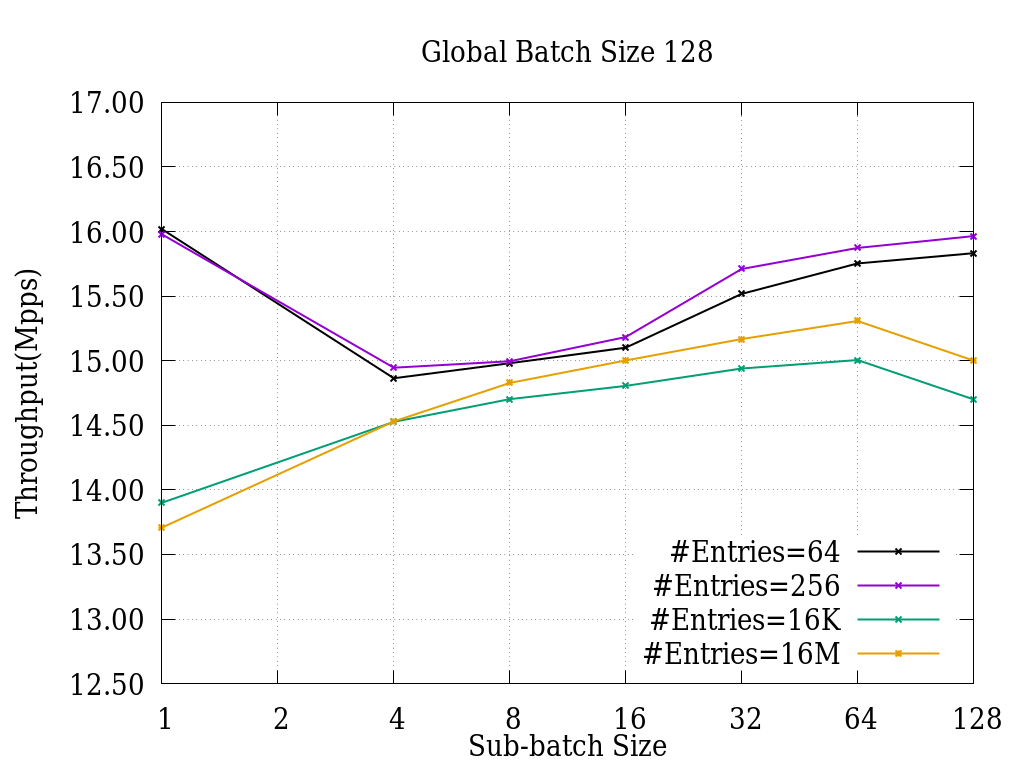
\includegraphics[width = \linewidth]{Figures/Subbatching.png}
\caption{The effect of sub-batch-size $b$ on application throughput, for four different configurations of the L2 forwarding application. We use batch-size $B=32$ for these experiments.}
\label{fig:subbatchfigure}
\end{figure}

\subsection{Sensitivity of Throughput to $b$}
To further understand the sensitivity of application throughput to the sub-batch-size $b$, we vary
$b$ for a fixed value of $B=128$, for the L2Fwd application. Figure~\ref{fig:subbatchfigure} plots
the results, again for different table-sizes. It is interesting to see
that if the table-size is less than, or equal to 256 entries, the throughput
{\em decreases} with increasing batch-size. On the other hand, if the table-size
is large (indicating that many table accesses will be cache misses), the
increasing sub-batch-size, generally improves throughput. If the sub-batch-size
is too large, (e.g., if it is 128 in this case), the performance usually dips
due to increased pressure on the caching subsystem, caused by the
increased memory footprint.

These results confirm that while sub-batching is useful for memory-bound
applications, it is not effective (or sometimes even harmful) for
compute-bound applications. We try and capture this formally in our
performance model, discussed next.

\subsection{Performance model}
We discuss a performance model to explain our experimental results. At a high-level,
the system can be modeled as a queueing network, with three parallel relevant
server components: namely,
the CPU, the CPU-memory interface, and the I/O-memory DMA interface. Assuming that
the three components
can execute in parallel, and have service rates $c$, $m$, and $d$, respectively, the
final throughput of the system would be:
$$
min(c, m, d)
$$
In other words, the throughput of the system is limited by the slowest component (each
packet is expected to traverse all three components).

With batching, we allow multiple in-flight packets on the DMA interface, and
hence increase the parallelism and service rate $d$. If the batch-size is $B$, then
the ideal improvement in the service rate of the DMA interface would be $B*d$ (i.e., linear
scaling).
However, in practice,
the interface is not fully parallelizable, and so the service rate of
the DMA interface increases as some function $f_{dma}(d, B)$. The plot in Figure~\ref{fig:tablesize}
can be used to roughly approximate the shape of this function $f_{dma}$ with increasing value of $B$.

Similarly, with sub-batching, we allow multiple in-flight memory requests on the
CPU-memory interface, and hence increase the service rate $m$. If the batch-size is $b$,
assume that the service rate of the CPU-memory interface is denoted by
a function $f_{mem}(m, b)$. The shape of $f_{mem}$ can be roughly approximated using
the plots in Figure~\ref{fig:subbatchfigure}. As we can see, the shape of both functions $f_{dma}$
and $f_{mem}$ are dependent on the characteristics of the application. For example,
if the application is compute-bound, $f_{mem}$ typically decreases with increasing $b$.
On the other hand, $f_{mem}$ increases with increasing $b$, for memory-bound applications,
if $b<128$.

Finally, if any improvements can be made to the CPU processing logic (e.g., see discussion
in Section~\ref{sec:discussion}), then those
are counted towards improvements in $c$. In summary, with batching and sub-batching, the
throughput of an application can be represented as:
$$
min(c, f_{dma}(m, b), f_{mem}(d, B))
$$

Thus, a compiler needs to first estimate the characteristics of the application. For example,
the compiler may run the application for different configurations in an offline
phase, to make conclusions about the degree of compute-boundedness ($c$), memory-boundedness ($m$),
and I/O-boundedness ($d$) of that application. Then, given a machine, the compiler may
use this information with the model
presented above to decide the optimal values for $b$ and $B$.

While our model is preliminary, it does provide an initial basis for reasoning about
performance while generating code for packet processing pipelines.

\subsection{Comparison with other related work}
\label{comparisonexperiment}
\begin{figure}[ht]
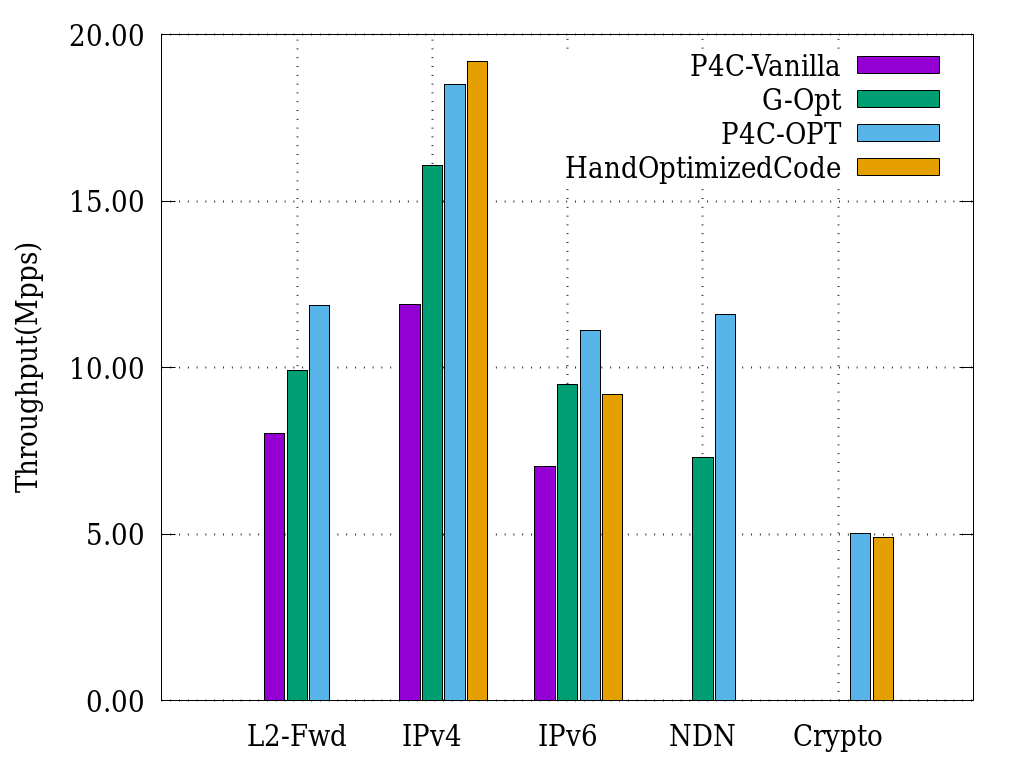
\includegraphics[width = \linewidth]{Figures/appscmp.png}
\caption{Comparison with other related work.}
\label{comparisonfigure}
\end{figure}
Figure \ref{comparisonfigure} compares our automatic generated code with vanilla P4C \cite{Laki:2016:HSP:2934872.2959080},
with another
related work, G-Opt, aimed at extracting memory-level parallelism through manual annotations \cite{189006},
and comparable
hand-optimized code available as a part of the DPDK distribution.
To ensure fair comparisons, we verify that the number of lookups and number of entries in the table(s) is same in all experiments.
In cases where a hand-optimized version or G-Opt results are not available,
the corresponding throughput bar is omitted.

Comparing with vanilla P4C, we obtain 48\%, 55\%, 57\%, and 46\% throughput improvements for L2Fwd, IPv4, IPv6, and NDN applications respectively.
The L2Fwd-crypto application shows minimum improvements, due to its compute-intensive nature.
%In the applications, they are not exploiting batching \& prefetching and just with these optimizations there is a huge improvement.
\\
G-Opt is a previous effort at bridging the gap between CPU and GPU performance for packet processing
applications. The G-Opt authors manually annotate code to identify expensive memory accesses and use
multithreading and context-switching to hide the memory latency. There are two important ways in which
our work differs from G-Opt: (1) our approach is largely automatic and works with a high-level
program representation. (2) we employ batching and sub-batching instead of multithreading, which
makes our approach more efficient as it avoids context-switching overheads.
We report a 20\%, 15\%, 17\%, and 59\% improvement over G-Opt for L2Fwd, IPv4, IPv6, and NDN applications respectively,
in head-to-head comparisons. We find that G-Opt authors did not systematically explore the space of
all possible transformations, when compared with our work, perhaps due
to the lack of a performance model. Our systematic exploration of $B$ and $b$, allows
us to maximize the throughput, beyond previous work.

Comparing with hand-optimized code available as a part of the DPDK distribution, we find that we are sometimes
slightly worse (4\% worse for IPv4), and sometimes significantly better (20\% better for IPv6). It is not
surprising that our compiler-based approach of systematic exploration across the parameter space can perform
better than hand-optimized code written by developers.

\subsection{Scalability}
\label{scalability}
\begin{figure}[ht]
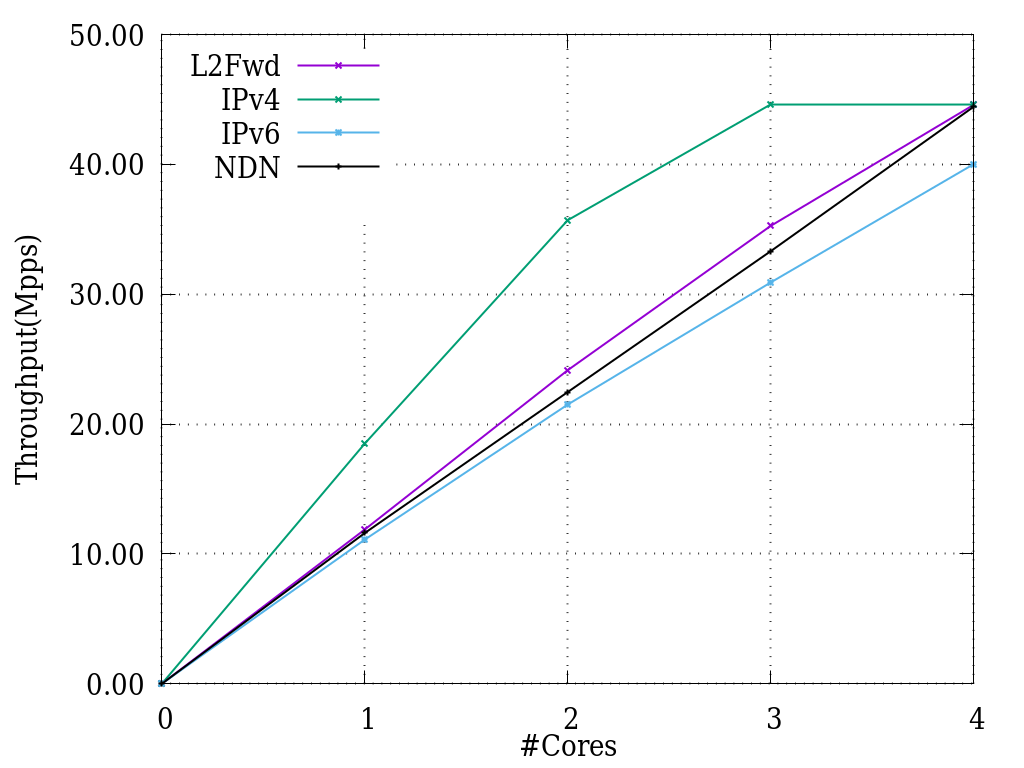
\includegraphics[width = \linewidth]{Figures/cores.png}
\caption{Number of Cores vs Throughput}
\label{cores}
\end{figure}
Figure \ref{cores} plots the application throughput with increasing number of cores.
Expectedly, the throughput usually scales linearly with the number of cores, except when
they saturate the PCIe bandwidth. In our experimental setup, the theoretical max achievable
throughput for 64 byte packets, summed across 4 NICs, is 59 Mpps (million packets per second). However, our
experimental results show that it cannot sustain this theoretical limit, and instead
saturates at 44Mpps. This difference between theoretical and observed throughputs,
is attributed to the fact that the same NICs are being used to both send and
receive packets, resulting in complex scheduling dependencies at the PCIe level.
IPv4 throughput hits the PCIe bandwidth limit in our experimental setup (the lookup algorithm for IPv4 is the fastest among all applications).
IPv6 packet throughput is slightly lower than others because it uses larger
(78-byte) packets.

\subsection{Latency}
In all our experiments, the end-to-end latency of a packet can be at most $B$ times worse than optimal. Usually, trading-off
increased latency (in an already fast end-to-end system) for better throughput, is acceptable for most real-world
applications.

\section{Discussion}
\label{sec:discussion}
While we restricted our discussion to batching and sub-batching, compiler
transformations can be much more sophisticated. For example, the choice
of data-structure to maintain and lookup the table, is often critical
to the CPU speed of the application.
We believe that existing
work in the realm of data-representation synthesis in programming languages
\cite{data_representation_synthesis, concurrent_data_representation_synthesis},
can be leveraged effectively in this setting. We discuss one such
experiment where we optimized the trie data structure used for IPv6 longest
prefix match, to reduce the number of average memory accesses per packet.

We implemented longest-prefix match lookup based on a compressed trie, and
experimented with our IPv6 application, albeit with
20,000 IPv6 prefixes, all having length 48.
We save around 1.25 memory accesses per packet for this application, resulting in 16\%
higher throughput. In general, the required transformations are highly dependent
on the application (e.g., L2 forwarding vs. IPv6 lookup), and the data (e.g.,
table size), and these characteristics could change over time.
We think that this argues for an automatic adaptive optimization engine, like the one
we have prototyped inside P4C, to be able to efficiently utilize the available hardware
resources.

\section{Related Work}
\label{relatedwork}
There has been a plethora of related work on CPU-based packet processing
and related programming models, including Click \cite{kohler2000click} and RouteBricks \cite{dobrescu2009routebricks}.
Manual optimizations to improve the performance of packet processing algorithms \cite{dobrescu2009routebricks, 189006, Kim:2012:PBC:2349896.2349910, Zhou:2013:SHP:2535372.2535379} have also been studied extensively.
In contrast, our work takes a compiler-centric approach to this problem, targeting micro-architectural
optimizations, by systematically exploring the space of potential configurations. Our results
show performance improvements over previous work. While our approach is aimed at automatic code generation from a high-level
specification, most previous works involved manual optimizations for individual applications. We have already compared our work
with some of the most relevant previous work through our experiments.

Previous work in compiler optimization has close parallels with our work too.
Shangri-La et. al. \cite{Chen:2005:SAH:1065010.1065038} generate an
optimized binary for a specialized {\em network processor}, and show that the generated binary works as
well as hand-tuned code. Dobrescu et. al. \cite{Dobrescu:2010:CPM:1921151.1921154} automate the decision
of splitting an application into parallel components to achieve high throughput. Previous work on
data-representation synthesis \cite{data_representation_synthesis, concurrent_data_representation_synthesis}
involves automatically inferring the optimal data structures and schedule for a high-level program
specification. Unlike this previous work, our focus on network processing pipelines on
general-purpose hardware enables more domain-specific optimizations and deeper micro-architectural modeling for better
overall performance.

While our initial efforts are aimed at optimization and performance modeling, we hope
to extend this work, towards developing an adaptive optimizing compiler for packet-processing pipelines.